\documentclass{thesis-ekf}
\usepackage[T1]{fontenc}
\PassOptionsToPackage{defaults=hu-min}{magyar.ldf}
\usepackage[magyar]{babel}
\usepackage{amssymb,amsthm,pdfpages}
\footnotestyle{rule=fourth}

\newtheorem{tetel}{Tétel}[chapter]
\theoremstyle{definition}
\newtheorem{definicio}[tetel]{Definíció}
\theoremstyle{remark}
\newtheorem{megjegyzes}[tetel]{Megjegyzés}

\begin{document}
	
	\institute{Matematikai és Informatikai Intézet}
	\title{Moduláris Plug \& Play IoT / okos~otthon rendszer}
	\author{Farkas Levente\\Program tervező informatikus BSc}
	\supervisor{Dr. Geda Gábor\\egyetemi docens}
	\city{Eger}
	\date{2025}
	\maketitle
	\tableofcontents
	\chapter*{Bevezetés}
	\addcontentsline{toc}{chapter}{Bevezetés}
	
	Az emberi faj a létezésétől kezdve lusta volt és lesz. Minden nap valamivel könnyebbé, egyszerűbbé akarjuk tenni a mindennapokat, hogy minél kevesebbel keljen foglalkoznunk és több időt tölthessünk más tevékenységgel. Az okos otthon rendszerek pontosan ezt teszik lehetővé, ezek régen drágák voltak így csak a tehetősebb emberek engedhették meg maguknak. Ma azonban olcsóbb ökoszisztémák is léteznek, de még így sem tudják sokan megfizetni. A projekt amiről ezen dolgozat szól egy olcsóbb, közösség alapú ökoszisztéma létrehozását tűzte ki célul.
	
	Számomra elképesztő belegondolni abba, hogy pár sor kóddal ki tudunk hatni a környezetünkre. Főképp azért, mert a programozás szempontjából én mindig adatkezelésként tekintettem a munkánkra. Még a szakdolgozat témájának kiválasztása előtt kapcsolatba kerültem a mikrokontrollerek világával és attól a ponttól nem tudtam elengedni ezen eszközök varázsát. Tekintettel arra, hogy az áramkörök és elektromosság foglalkoztatott hobbi szinten már régóta, ez egy nagyszerű lehetőség volt, hogy kettő nagy szenvedélyemet, az informatikát és az áramköröket ötvözzem a szakdolgozatomban. Számomra hihetetlen volt akár csak egy LED\footnote{Light Emitting Diode, avagy fényt kibocsájtó dióda.} villanása is.
	
	Szakdolgozatom termék-orientált. Célja az, hogy a kevésbé tehetős emberek számára is elérhetővé tegye az okos otthonok varázsát. Logikám szerint az okos eszközök árát nagyrészt a programozható mikrochipek teszik ki, ezeknek egy részről a hozzá tartozó áramkört kell vezérelniük, amely nem egy nehéz feladat, azonban az adatnak amely alapján ez működni fog valahogy el kell jutnia az eszközhöz, ez WiFi-n keresztül történik minden esetben, azonban így jelentősen megugrik ezek ára. A gondolatmenetemben egy egy eszközt képzeltem el, amely ezt a drága technológiát központosítja, ezzel a rendszer szummázott árát csökkentve.
	
	Az eszköz önmagában nem képes sok mindenre, azonban a hozzá kapcsolódó ,,buta'' modulok használatával lehetőség nyílik arra, hogy egy eszköz négy modult, azaz működésében különálló okos eszközt kezeljen.
	A fejlesztés idejében az eszköz négy modult képes befogadni, azonban ez áramkör és program módosítással növelhető.
	\chapter{Technológiák}
	\chapter{ESP32, az eszköz}
	\section{ESP32 bemutatása}
	Az ESP32 egy rendkívül sokoldalú és hatékony mikrokontroller, amely számos területen alkalmazható. Duális magos processzora, integrált Wi-Fi és Bluetooth képességei, valamint gazdag I/O lehetőségei miatt kiváló választás mind IoT, mind ipari vagy okos otthon alkalmazásokhoz. Az ESP32 fejlesztése egyszerű és gyors, köszönhetően a széles körben elérhető fejlesztői eszközöknek és könyvtáraknak. Ezek a tulajdonságok teszik az ESP32-t az egyik legnépszerűbb mikrokontrollerré a beágyazott rendszerek világában.
	
	Az általam \aref{img_myesp} használt modell az ESP32-S3-DevKitC-1 N32R8V, amely egy ESP32-S3-WROOM-2 chipet tartalmaz, ezt az Espressif System fejlesztette ki.
	\begin{figure}[!ht]
		\centering
		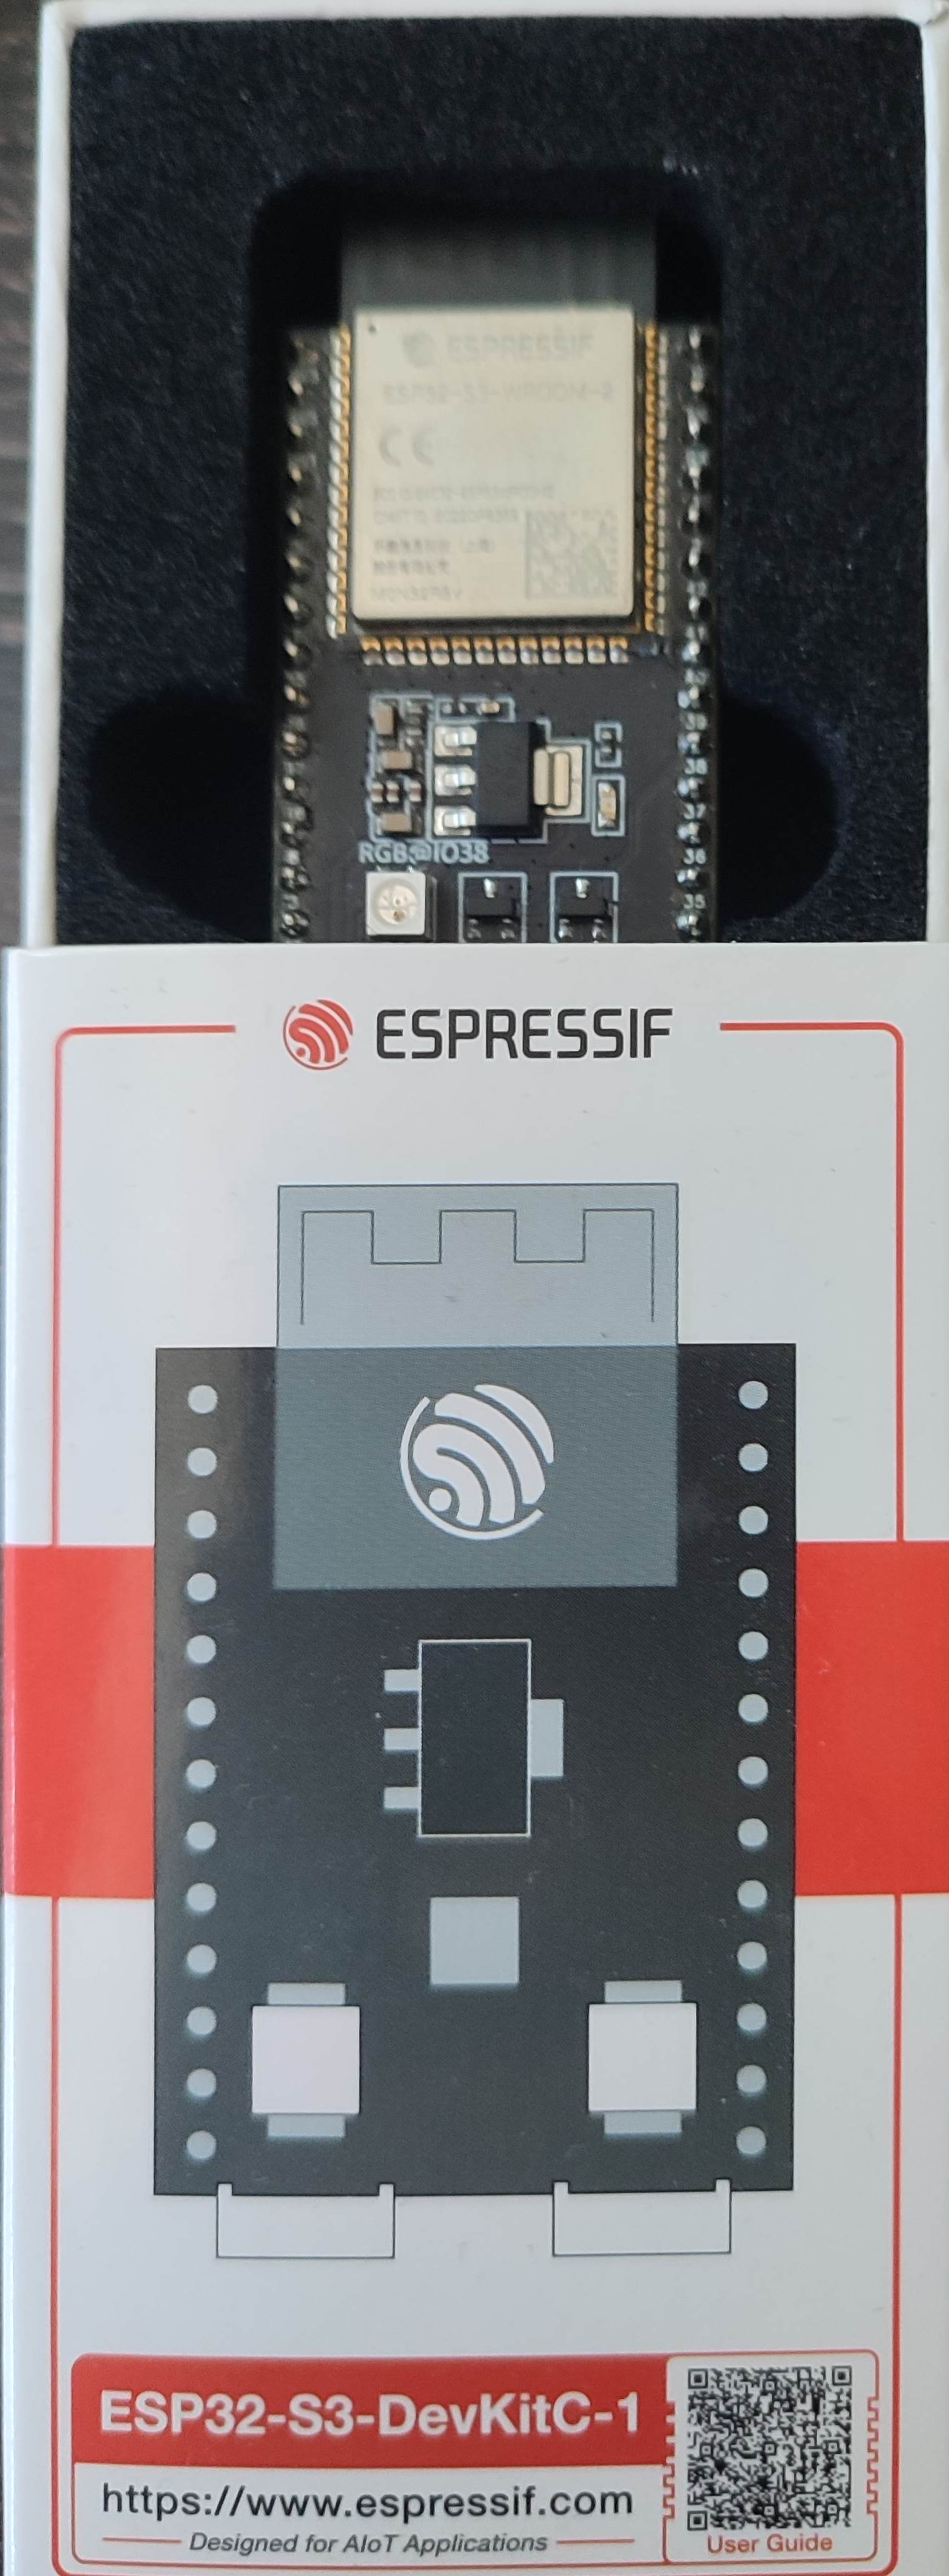
\includegraphics[width=3cm]{MyESP32}
		\caption{Általam használt ESP32 modell}
		\label{img_myesp}
	\end{figure}
	
	Ezen eszközök számos bemeneti és kimeneti perifériákkal rendelkeznek:
	\begin{itemize}
		\item Digitális I/O pin-ek
		\item Analóg bemenetek (ADC\footnote{Analog to Digital Converter, lehetővé teszi az áramkörben érzékelt analóg jelek feldolgozását.})
		\item Digitális-analóg átalakítók (DAC\footnote{Digital to Analog Converter, lehetővé teszi az áramkörre kibocsájtott feszültség modulálását.})
		\item PWM (Pulse Width Modulation\footnote{Ezen technológia teszi lehetővé a DAC működését.}) kimenetek
		\item SPI, I2C, UART kommunikációs interfészek
	\end{itemize}
	Ezek a csatlakozók lehetővé teszik különböző érzékelők, kijelzők és egyéb perifériák csatlakoztatását.
	\section{Fejlesztés}
	\subsection{Hardver szintű fejlesztés}
	A projekt megvalósításához szükség volt egy egyedi áramkörre, amivel maximalizálhatom az elérhető portok számát.
	\begin{figure}[!ht]
		\centering
		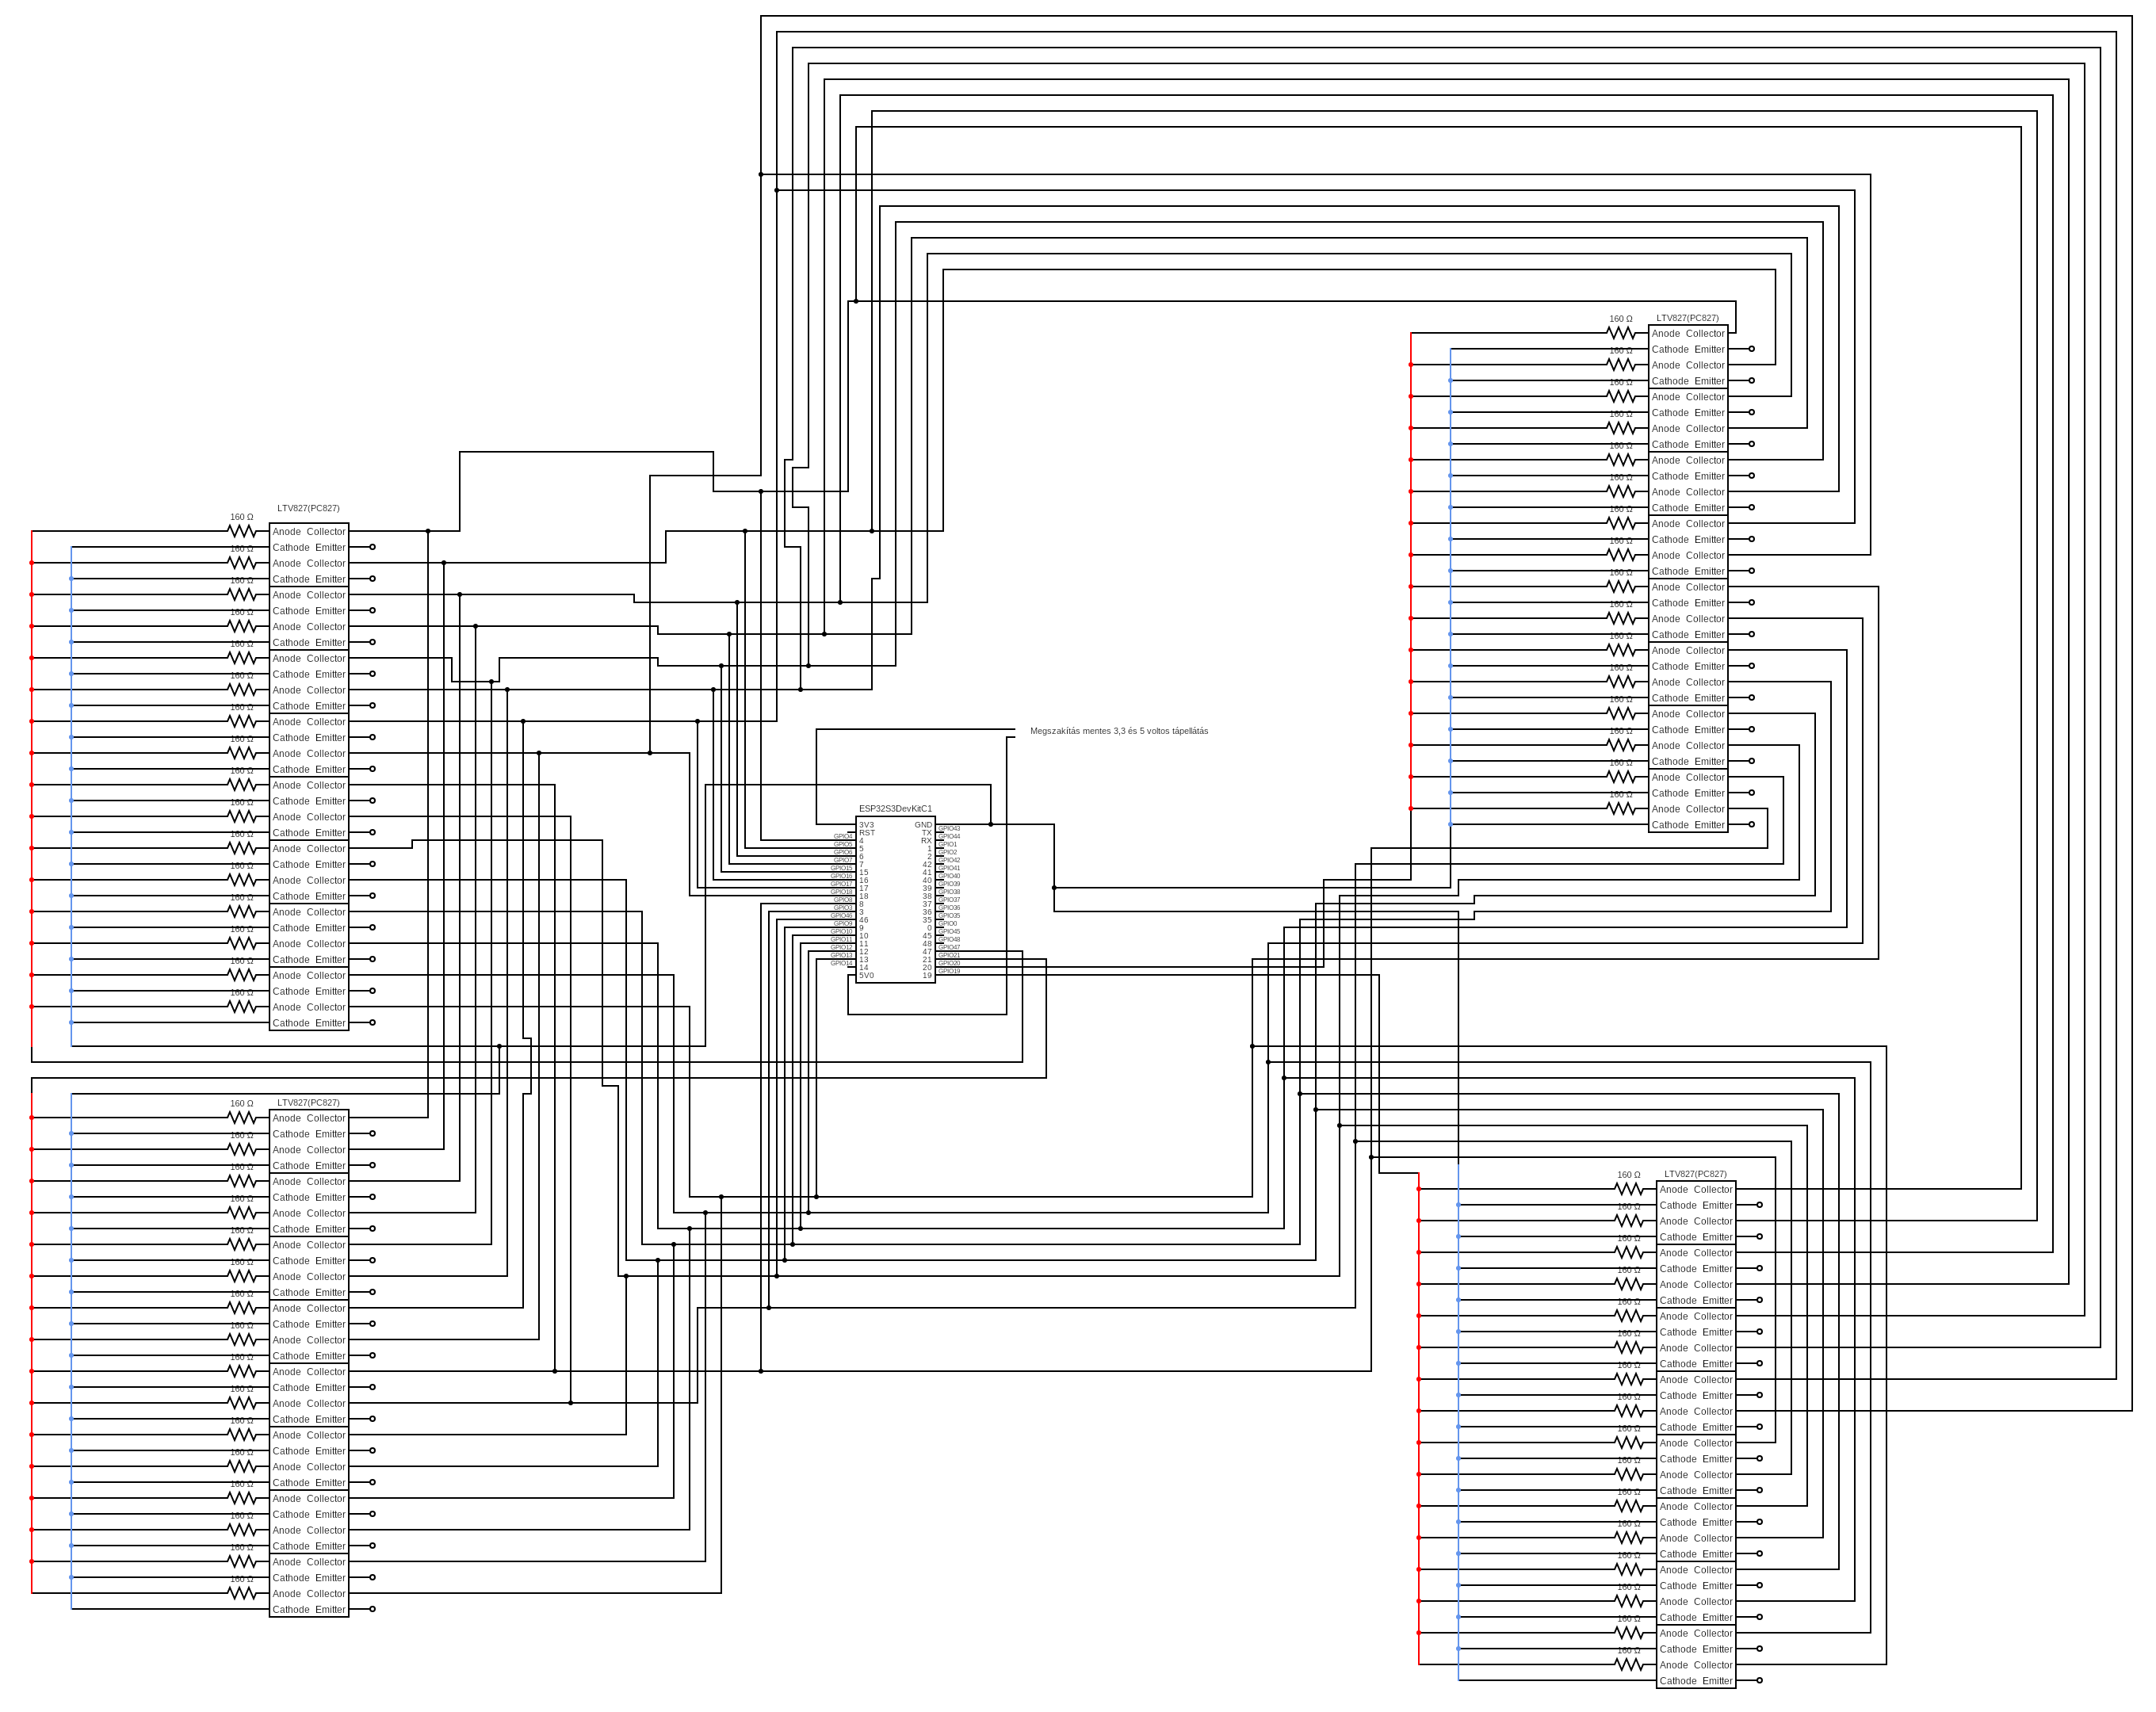
\includegraphics[width=10cm]{circuit}
		\caption{Egyedi áramkör}
		\label{img_circ}
	\end{figure}
	A \ref{img_circ}-es ábrán látható az említett áramkör, amely segítségével elérem az általam elfogadható eredményt. Ebben a fő alkatrész az optocsatoló, amellyel igyekeztem  az esetleges interferenciát csökkenteni.
	
	Ez a diagram a Circuit Diagram\footnote{ \url{https://www.circuit-diagram.org/}} segítségével készült.
	Az ábra nem tartalmazza az érzékelő vezetékeket, amivel az eszköz érzékeli, hogy csatlakoztatva van-e a modul.
	\subsection{szoftver fejlesztése}
	\chapter{API}
	
	\chapter{Front end}
\end{document}